\documentclass[a4paper, 12pt]{article}

\usepackage{enumerate}
\usepackage{hyperref}
\hypersetup{
	colorlinks=true,
	linkcolor=blue,
	filecolor=blue,
	urlcolor=blue,
	citecolor=blue,
}
\usepackage{amsmath}
\usepackage{amsthm}
\usepackage{amssymb}
\usepackage[margin=3cm]{geometry}
\usepackage{mathpazo}
\usepackage{url}
\usepackage{subcaption}
\usepackage{tikz}
\usepackage{pgf}
\usepackage{longtable}
\usepackage{multirow}
\usepackage{graphicx}
\usepackage{pgfplots}
\usepackage{cleveref}
\usepackage{bbm}
\usepackage{wrapfig}
\usepackage{mathrsfs}
\usepackage{afterpage}
\usepackage[svgnames]{xcolor}
\usepackage{newverbs}

\numberwithin{equation}{section}
\numberwithin{figure}{section}

\newtheorem{thm}{Theorem}[section]
\newtheorem*{thm*}{Theorem}
\newtheorem*{con*}{Conjecture}
\newtheorem{lem}[thm]{Lemma}
\newtheorem{prop}[thm]{Proposition}
\newtheorem{cor}[thm]{Corollary}
\newtheorem{lemma}[thm]{Lemma}
\newtheorem{conj}[thm]{Conjecture}

\theoremstyle{definition}
\newtheorem{defn}[thm]{Definition}
\newtheorem{remark}[thm]{Remark}
\newtheorem{ex}[thm]{Example}
\newtheorem{quest}[thm]{Question}
\newtheorem{obs}[thm]{Observation}

\renewcommand{\leq}{\leqslant}
\renewcommand{\geq}{\geqslant}
\newcommand{\N}{\mathbb{N}}
\newcommand{\Z}{\mathbb{Z}}
\newcommand{\Q}{\mathbb{Q}}
\newcommand{\R}{\mathbb{R}}
\newcommand{\C}{\mathbb{C}}
\newcommand{\define}[1]{\textit{\textbf{#1}}}

\setcounter{tocdepth}{2}

\allowdisplaybreaks

\title{Software for Mathematical Scientists and Educators}
\author{Joshua Maglione}
\date{\today}

\begin{document}

\maketitle
\tableofcontents

\section*{Introduction}

Communicating mathematics and performing long computations are both vitally
important and challenging. Thankfully there is a wide selection of software to
make these tasks more manageable. In this module, we will explore software used
by everyday mathematicians and scientists. These include biologists, chemists,
computer scientists, data scientists, financial analysts, educators, engineers,
and physicists. 

The goal is to build a foundation by using some of the most ubiquitous software
in the field. This will help students throughout their career in and out of
university. We will cover four topics in this module:
\begin{enumerate} 
	\item Mathematical Typesetting and \LaTeX,
	\item Python and Jupyter Notebooks,
	\item Introduction to Programming,
	\item Symbolic Computation and SageMath.
\end{enumerate}


\section{Mathematical Typesetting and \LaTeX}

With advances in printing and typesetting, the question of how to produce
high-quality mathematical symbols and texts is challenging. Without going
through the history, we now have essentially two main styles of software to
write mathematical formulae, diagrams, and images:
\begin{enumerate}
	\item What-You-See-Is-What-You-Get (WYSIWYG) and
	\item typesetting software (or write-format-preview style).
\end{enumerate}

Software like Microsoft Word, Apple Pages, or LibreOffice Writer are WYSIWYG
editors because you see and edit the document as a final product (regardless of
whether or not it is the final product). This remove the user from having to
remember commands for the document layout, and it has a lower barrier of entry,
which is one of its strongest advantages. However, this is not the norm for
professionals using many mathematical symbols, and the primary disadvantage to
these kinds of software is their sluggish pace. 

One of the first typesetting software for mathematics is \TeX---if not
\textit{the} first. It was written by Donald Knuth\footnote{You can read Knuth's
original memo describing \TeX. He called the memo the ``Preliminary preliminary
description of TEX''~\cite{TeX-draft}.} in 1978~\cite{Knuth-Quanta}, and it is
the cornerstone of the more modern software \LaTeX\ written by Leslie Lamport in
1986~\cite{Lamport}. Although \TeX\ is still used today, \LaTeX\ is far more
popular. The primary disadvantage to these systems is the higher barrier to
entry, but the over-powering advantage is the speed with which one can produce
beautiful and high-quality mathematical symbols. Both \TeX\ and \LaTeX\ are free
and open-source software. 

As alluded to previously, these are typesetting software, so a user writes in a
markup language, usually in a \texttt{tex}-file; then the user compiles the
file, and a \texttt{pdf}-file is produced. There are other options for output,
but this will be sufficient for us. Another asset is that one can import third
party \LaTeX\ packages to perform more specialized tasks. We will become
familiar with basic \LaTeX\ formatting and use some packages to help construct
beautiful documents. 

For web-based mathematical symbols, MathJax~\cite{MathJax} is primarily used.
However, there is a new, much faster, alternative called KaTeX~\cite{KaTeX}.
Currently, KaTeX can only do a (proper) subset of what MathJax can do, but KaTeX
does enough for everything I have needed for my website. 

\subsection{How to get \LaTeX}

This will not fully cover how to install \LaTeX\ on your own machine, but
hopefully it gives you enough information to help you. It not that \LaTeX\
updates so frequently---in fact \LaTeX\ is still on its second edition
(formatted as \LaTeXe)---it is that packages tend to update or just need
installation. 

For Windows machines, I would recommend MiKTeX. This install LaTeX and comes
with a package manager to help with package installation. A similar version is
available on Mac OS, and it is called MacTeX. Both MiKTeX and MacTeX have
graphical user interfaces. For Linux systems, TeX Live is what I recommend, and
it usually comes pre-installed. It has its own package manager invoked by the
command \texttt{tlmgr}. 

\subsection{Workflow and document structure}

The basic workflow is perhaps only a little more complicated than how it might
be for WYSIWYG software. Here is the basic workflow. 
\begin{enumerate}
	\item Create a \texttt{tex}-file and write \LaTeX\ markup. 
	\item Compile the \texttt{tex}-file with the command \texttt{pdflatex}.
	\item Sometimes errors are raised and need to be addressed. If no errors
	arise, then a \texttt{pdf}-file is created (or overwritten).
	\item View and review the output \texttt{pdf}-file. 
\end{enumerate}
With the exception of the initial creation of the file, all of these steps are
repeated often. How often? That depends on you and your situation. I would
recommend that, when addressing bugs or typos, that one compile often and review
carefully what has changed. 

The basic format of a \LaTeX\ document is simple. There are three commands that
must be present, and often one tries to adhere to some logical structure due to
collaborations or just to readability over longer periods of time. The first
command that appears in a functioning \texttt{tex}-file is the following:
\begin{verbatim}
			\documentclass[<options>]{<style>}
\end{verbatim}
where \texttt{<style>} is replaced with the name of the desired document class
and \texttt{<options>} is replaced with optional parameters for the specific
document class. For example, this current \texttt{pdf} document was built using
\begin{verbatim}
			\documentclass[a4paper, 12pt]{article}
\end{verbatim}
Some other popular document classes, besides \texttt{article}, are 
\begin{itemize}
	\item \texttt{beamer} : for slides,
	\item \texttt{book} : for books,
	\item \texttt{letter} : for letters,
	\item \texttt{standalone} : often used with the package \texttt{TikZ} for
	stand alone pictures.
\end{itemize}
There are also AMS-inspired article and book classes: \texttt{amsart} and
\texttt{amsbook} and KOMA-script versions: \texttt{scrartcl}, \texttt{scrbook},
\texttt{scrlttr2}, and \texttt{scrreprt}. The other two required commands are 
\begin{verbatim}
			\begin{document}
			\end{document}
\end{verbatim}
which encapsulate the main body of the \texttt{tex}-file. \Cref{fig:tex-file}
shows the basic layout of a \texttt{tex}-file.

\begin{figure}[h]
	\centering
	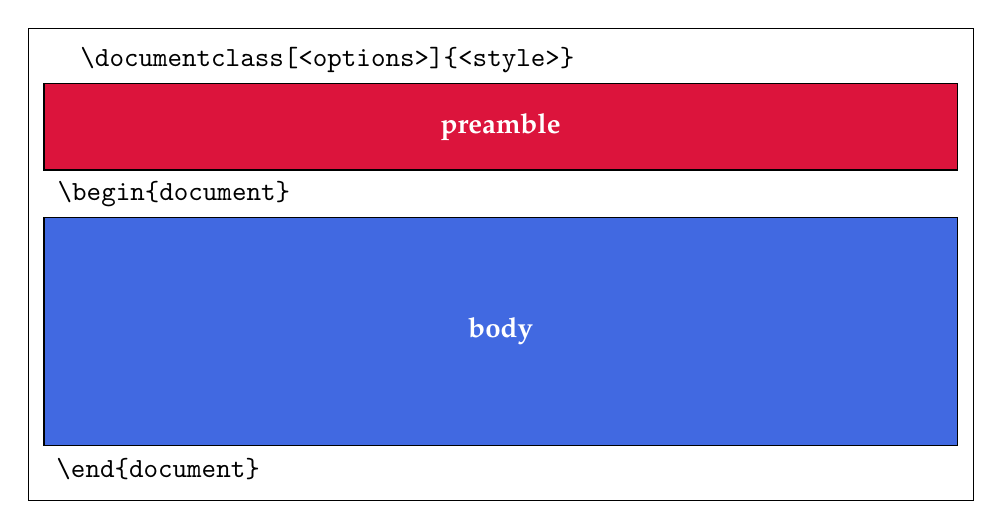
\begin{tikzpicture}
		\draw (0,-1) rectangle (12,5);
		\draw[fill=Crimson] (0.2, 3.2) rectangle (11.8, 4.3);
		\draw[fill=RoyalBlue] (0.2, -0.3) rectangle (11.8, 2.6);
		\node at (3.8,4.6) {\verb_\documentclass[<options>]{<style>}_};
		\node at (1.85,2.9) {\verb_\begin{document}_};
		\node at (1.65,-0.6) {\verb_\end{document}_};
		\node[White] at (6, 3.75) {\textbf{preamble}};
		\node[White] at (6, 1.15) {\textbf{body}};
	\end{tikzpicture}
	\caption{Basic structure of a \texttt{tex} file.}
	\label{fig:tex-file}
\end{figure}

\subsection{Source files}

\LaTeX\ \define{source files} are the necessary files needed to compile a
\texttt{tex} file. In particular, a \texttt{tex} file need not be self
contained; there are many reasons why this might be the case. For example, one
might embed graphics in the form of \texttt{jpeg} or \texttt{png} files, or one
might use \textsc{Bib}\TeX\ to dynamically format their bibliography---more on
this in \Cref{sec:bibtex}.

In the process of compiling a \texttt{tex} file to a \texttt{pdf} file, \LaTeX\
produces several auxillary files. These serve specific purposes, but their
particular uses are outside of the scope we will explore. Because so many
additional files are created in the compilation process, it is usually preferred
to build a directory for each \LaTeX\ project. For example, the file names in
the directory for these lecture notes can be seen in \Cref{fig:all-files}.

\begin{figure}[h]
	\centering 
	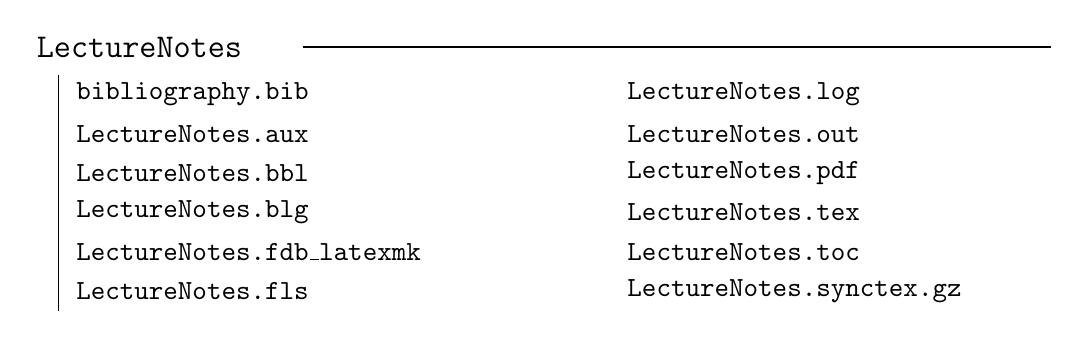
\begin{tikzpicture}
		\node[anchor=west] at (-0.5,3.1) {{\large\texttt{LectureNotes}}};
		\node[anchor=west] at (0,2.5) {\texttt{bibliography.bib}};
		\node[anchor=west] at (0,2) {\texttt{LectureNotes.aux}};
		\node[anchor=west] at (0,1.5) {\texttt{LectureNotes.bbl}};
		\node[anchor=west] at (0,1) {\texttt{LectureNotes.blg}};
		\node[anchor=west] at (0,0.5) {\texttt{LectureNotes.fdb\_latexmk}};
		\node[anchor=west] at (0,0) {\texttt{LectureNotes.fls}};
		\node[anchor=west] at (7,2.5) {\texttt{LectureNotes.log}};
		\node[anchor=west] at (7,2) {\texttt{LectureNotes.out}};
		\node[anchor=west] at (7,1.5) {\texttt{LectureNotes.pdf}};
		\node[anchor=west] at (7,1) {\texttt{LectureNotes.tex}};
		\node[anchor=west] at (7,0.5) {\texttt{LectureNotes.toc}};
		\node[anchor=west] at (7,0) {\texttt{LectureNotes.synctex.gz}};
		\draw (-0.1, 2.75) -- (-0.1, -0.25);
		\draw (3, 3.1) -- (12.5, 3.1);
	\end{tikzpicture}
	\caption{The files in the \texttt{LectureNotes} directory.}
	\label{fig:all-files}
\end{figure}

The only files necessary to compile in \Cref{fig:all-files} are
\texttt{LectureNotes.tex} and \texttt{bibliography.bib}. The rest of the files
are produced by the compilation process. 




\subsection{An introduction to \LaTeX\ syntax}

We will not cover all of the \LaTeX\ syntax here. When we discuss mathematical
symbols and formulae in \Cref{sec:latex-math}, we will cover more. There are
some symbols that \LaTeX\ redefines. For example, \% indicates that the rest of
the line should be ignored by the compiler:
\begin{verbatim}
			% This is a comment and will be ignored by the LaTeX compiler.
\end{verbatim}

Commands in \LaTeX\ start with the \verb_\_ symbol. We have already seen
examples of this with the following commands:
\begin{verbatim}
			\documentclass[a4paper, 12pt]{article}
			\begin{document}
			\end{document}
\end{verbatim}
Arguments are input using the \verb_{_ and \verb_}_ symbols, and multiple
arguments would require multiple sets of \verb_{_ and \verb_}_. Optional
parameters are input using the \verb_[_ and \verb_]_ symbols, but multiple
optional parameters are listed within the single use of \verb_[_ and \verb_]_
separated by commas. Not every command requires input arguments; for example, to
format LaTeX as \LaTeX, one uses the command .

\subsection{Dynamic bibliographies and \textsc{Bib}\TeX}
\label{sec:bibtex}


\subsection{Mathematical symbols and formulae}
\label{sec:latex-math}


\subsection{\LaTeX\ Environments}
\label{sec:latex-envs}


\subsection{Some \LaTeX\ packages}
\label{sec:latex-packages}




\newpage

\bibliography{bibliography}
\bibliographystyle{plain}

\end{document}